\documentclass[a4paper,12pt]{article}

\usepackage[
    left=2cm,
    right=2cm,
    top=3cm,
    bottom=3cm
]{geometry}

\usepackage[utf8]{inputenc}
\usepackage[czech]{babel}
\usepackage[T1]{fontenc}
\usepackage{graphicx}
\usepackage{array}
\usepackage{booktabs}
\usepackage{tabularx}
\usepackage{makecell}
\usepackage{float}
\usepackage{newunicodechar}
\usepackage{url}
\usepackage{siunitx}
\usepackage{listings}
\usepackage{xcolor}
\usepackage{diagbox}
\usepackage{hyperref}
\usepackage{tikz}
\usepackage{pgfplots}
\usepgfplotslibrary{polar}
\pgfplotsset{compat=1.18}

\usepackage{fancyhdr}
\pagestyle{fancy}

\fancyhf{}
\fancyhead[L]{SME -- Lab 10: Měření na transformátorech}
\fancyhead[R]{Pavel Pernička}
\fancyfoot[C]{\thepage}

\fancypagestyle{firstpage}{
    \fancyhf{}
    \renewcommand{\headrulewidth}{0pt}
    \renewcommand{\footrulewidth}{0pt}
    \fancyfoot[C]{\thepage}
}

\definecolor{myblue}{RGB}{111,0,248}
\newcommand{\colorcircle}[1]{%
  \tikz[baseline=-0.6ex]\draw[fill=#1,draw=none] (0,0) circle (1.5ex);%
}
\newcommand{\unitC}{\,^\circ\mathrm{C}}
\newcommand{\unitV}{\,\mathrm{V}}
\newcommand{\unitA}{\,\mathrm{A}}
\newcommand{\units}{\,\mathrm{s}}
\newcommand{\unitmin}{\,\mathrm{min}}

\newcommand{\centered}[1]{\begin{tabular}{l} #1 \end{tabular}}

\addto\captionsczech{\renewcommand{\refname}{Seznam použité literatury}}
\addto\captionsczech{\renewcommand{\figurename}{\textbf{Obrázek}}}
\addto\captionsczech{\renewcommand{\tablename}{\textbf{Tabulka}}}
\renewcommand{\lstlistingname}{\textbf{Kód}}

\lstset{
    language=Python,
    basicstyle=\ttfamily\footnotesize,
    keywordstyle=\color{blue},
    commentstyle=\color{gray},
    stringstyle=\color{red},
    numbers=left,
    numberstyle=\tiny\color{gray},
    stepnumber=1,
    breaklines=true,
    frame=single
}

\begin{document}
\thispagestyle{firstpage}

\vspace*{\fill}
\begin{center}
\renewcommand{\arraystretch}{1.75}

\begin{tabularx}{\textwidth}{|X|X|X|}
    \hline
    \multicolumn{1}{|c|}{\rule{0pt}{2.25cm} 
\includegraphics[height=2cm]{img/ctu_logo.png}}
    & \multicolumn{2}{c|}{\makecell{\textbf{KATEDRA MĚŘENÍ}}} \\
    \hline
    \multicolumn{3}{|c|}{\Large \textbf{\centered{Senzory a měření}}} \\
    \hline
    \multicolumn{2}{|X}{\small{Jméno} \newline \textbf{Pavel Pernička}}
    & \multicolumn{1}{|X|}{\small{Datum měření} \newline \textbf{8.4.2026}} \\
    \hline
    {\small{Semestr} \newline \textbf{Letní 2026}}
    & {\small{Ročník} \newline \textbf{2.}}
    & {\small{Datum odevzdání} \newline \textbf{15.4.2026}} \\
    \hline
    \multicolumn{3}{|c|}{\rule{0pt}{1cm}} \\
    \hline
    \multicolumn{1}{|X|}{\small{Číslo úlohy \newline \textbf{10}}}
    & \multicolumn{2}{|p{9cm}|}{\small{Název úlohy \newline \textbf{Měření na transformátorech}}} \\
    \hline
\end{tabularx}

\end{center}
\vspace*{\fill}

\newpage
\pagestyle{fancy}
\section{A -- Měření rozptylového magnetického pole transformátoru}
\subsection{Domácí příprava}
\begin{itemize}
  \item Jaký senzor je vhodný pro měření maximální hodnoty indukce střídavého magnetického pole?
    \begin{itemize}
      \item Indukční cívka
    \end{itemize}
  \item Jaká hodnota výstupního napětí u tohoto senzoru (střední, efektivní nebo maximální) odpovídá maximální hodnotě magnetické indukce?
    \begin{itemize}
      \item Maximální hodnotě indukce odpovídá aritmetická střední hodnota napětí indukovaného v měřicí cívce po dvoucestném usměrnění.
    \end{itemize}
\end{itemize}

\subsection{Měření}
\subsubsection{Rezonanční kmitočet cívky}
Určete rezonanční kmitočet snímací cívky. Posuďte, zda ji lze použít pro měření dle bodů 2~a~3.
\par\noindent\rule{\textwidth}{0.4pt}

Rezonanční kmitočet určíme tak, že pomocí generátoru funkcí pouštíme do cívky sinusový průběh s postupně se měnící frekvencí. Pozorujeme proud tekoucí obvodem. Rezonanční kmitočet se nachází tam, kde má proud své minimum. U naší cívky jsme naměřili
$$
f_r = 2,9\ kHz
$$
Jelikož je $f_r$ řádově vyšší, než je síťová frekvence $50\ Hz$, nebude nám při měření dělat problémy.

\subsubsection{Indukce rozptylového magnetického pole -- Jádro EI}
Změřte orientačně indukci rozptylového magnetického pole transformátoru s jádrem EI. 
\par\noindent\rule{\textwidth}{0.4pt}
Naměřili jsme data uvedená v tabulce a dopočítali jsme z nich $B_{tan}$, $B_{rad}$ a $B_{celk} = \sqrt{B_{tan}^2 + B_{rad}^2}$ podle vztahu:
$$
B_m = \frac{U_s}{4\cdot f \cdot S \cdot N}
$$

kde $f=50\ Hz$ je síťová frekvence a závitová plocha $N\cdot S = 11,6\ m^2$ ze zadání. Napětí $U_{eff}$ převedeme na $U_s$ pomocí: $U_s = \frac{2\sqrt{2}}{\pi} U_{ef}$.

\begin{table}[H]
\centering
\scriptsize
\begin{tabular}{|c|c|c|c|c|c|c|c|c|c|c|c|c|c|}
\hline
$\varphi\ [^\circ]$ 
& 0 & 30 & 60 & 90 & 120 & 150 & 180 & 210 & 240 & 270 & 300 & 330 \\
\hline
$U_{tan}\ [\mathrm{V}]$ 
& $0,054$ & $0,046$ & $0,022$ & $0,003$ & $0,019$ & $0,041$ & $0,046$ & $0,036$ & $0,016$ & $0,003$ & $0,027$ & $0,045$ \\
\hline
$U_{rad}\ [\mathrm{V}]$ 
& $0,004$ & $0,006$ & $0,013$ & $0,014$ & $0,010$ & $0,002$ & $0,010$ & $0,025$ & $0,029$ & $0,029$ & $0,025$ & $0,015$ \\
\hline
$B_{tan}\ [\mathrm{mT}]$ 
& $0,021$ & $0,018$ & $0,009$ & $0,001$ & $0,007$ & $0,016$ & $0,018$ & $0,014$ & $0,006$ & $0,001$ & $0,010$ & $0,017$ \\
\hline
$B_{rad}\ [\mathrm{mT}]$ 
& $0,002$ & $0,002$ & $0,005$ & $0,005$ & $0,004$ & $0,001$ & $0,004$ & $0,010$ & $0,011$ & $0,011$ & $0,010$ & $0,006$ \\
\hline
$B_{celk}\ [\mathrm{mT}]$ 
& $0,021$ & $0,018$ & $0,010$ & $0,006$ & $0,008$ & $0,016$ & $0,018$ & $0,017$ & $0,013$ & $0,011$ & $0,014$ & $0,018$ \\
\hline
\end{tabular}
\caption{Magnetická indukce v různých úhlech okolo transformátoru s EI jádrem}
\end{table}

\begin{figure}[H]
\centering
\begin{tikzpicture}
\begin{polaraxis}[
    width=8cm,
    height=8cm,
    grid=both,
    ymin=0,
    ymax=0.025,
    ytick={0,0.005,0.010,0.015,0.020,0.025},
    xtick={0,30,60,90,120,150,180,210,240,270,300,330},
    xticklabels={0,30,60,90,120,150,180,210,240,270,300,330},
    yticklabel style={font=\scriptsize},
    xticklabel style={font=\scriptsize},
    yticklabel pos=upper,
    legend style={
        at={(1.2,0.5)},
        anchor=west,
        draw=none,
        font=\small
    }
]

\addplot[
    color=red,
    mark=square*,
    thick
] coordinates {
    (0,0.021) (30,0.018) (60,0.009) (90,0.001)
    (120,0.007) (150,0.016) (180,0.018) (210,0.014)
    (240,0.006) (270,0.001) (300,0.010) (330,0.017)
    (360,0.021)
};

\addplot[
    color=blue,
    mark=*,
    thick
] coordinates {
    (0,0.002) (30,0.002) (60,0.005) (90,0.005)
    (120,0.004) (150,0.001) (180,0.004) (210,0.010)
    (240,0.011) (270,0.011) (300,0.010) (330,0.006)
    (360,0.002)
};

\addplot[
    color=green!60!black,
    mark=triangle*,
    thick
] coordinates {
    (0,0.021) (30,0.018) (60,0.010) (90,0.006)
    (120,0.008) (150,0.016) (180,0.018) (210,0.017)
    (240,0.013) (270,0.011) (300,0.014) (330,0.018)
    (360,0.021)
};

\legend{$B_{tan}$,$B_{rad}$,$B_{celk}$}

\end{polaraxis}
\end{tikzpicture}
\caption{Znázornění magnetické indukce v různých úhlech okolo transformátoru s EI jádrem}
\end{figure}

\subsubsection{Indukce rozptylového magnetického pole -- toroidální transformátor}
Ověřte potlačení rozptylového magnetického pole u toroidního transformátoru. Otáčením transformátoru vyhledejte maximum pole v poloze „1“ a srovnejte ho s maximem pole u transformátoru EI. 
\par\noindent\rule{\textwidth}{0.4pt}

\begin{table}[H]
\centering
\scriptsize
\begin{tabular}{|c|c|c|c|c|c|c|c|c|c|c|c|c|c|}
\hline
$\varphi\ [^\circ]$ 
& 0 & 30 & 60 & 90 & 120 & 150 & 180 & 210 & 240 & 270 & 300 & 330 \\
\hline
$U_{tan}\ [\mathrm{V}]$ 
& $0,002$ & $0,002$ & $0,002$ & $0,003$ & $0,003$ & $0,003$ & $0,004$ & $0,004$ & $0,003$ & $0,003$ & $0,002$ & $0,002$ \\
\hline
$U_{rad}\ [\mathrm{V}]$ 
& $0,004$ & $0,004$ & $0,004$ & $0,003$ & $0,004$ & $0,003$ & $0,003$ & $0,003$ & $0,003$ & $0,004$ & $0,004$ & $0,004$ \\
\hline
$B_{tan}\ [\mathrm{mT}]$ 
& $0,0008$ & $0,0008$ & $0,0008$ & $0,0012$ & $0,0012$ & $0,0012$ & $0,0016$ & $0,0016$ & $0,0012$ & $0,0012$ & $0,0008$ & $0,0008$ \\
\hline
$B_{rad}\ [\mathrm{mT}]$ 
& $0,0016$ & $0,0016$ & $0,0016$ & $0,0012$ & $0,0016$ & $0,0012$ & $0,0012$ & $0,0012$ & $0,0012$ & $0,0016$ & $0,0016$ & $0,0016$ \\
\hline
$B_{celk}\ [\mathrm{mT}]$ 
& $0,0017$ & $0,0017$ & $0,0017$ & $0,0016$ & $0,0019$ & $0,0016$ & $0,0019$ & $0,0019$ & $0,0016$ & $0,0019$ & $0,0017$ & $0,0017$ \\
\hline
\end{tabular}
\caption{Magnetická indukce v různých úhlech okolo toroidálního transformátoru}
\end{table}

Maximum v poloze „1“ se zde vyskytuje při úhlech $120^\circ$, $180^\circ$, $210^\circ$ a $270^\circ$ o hodnotě přibližně $0,0019\ \mathrm{mT}$. U předchozího transformátoru je maximální hodnota větší, přibližně $0,021\ \mathrm{mT}$ při úhlu $0^\circ$. Vidíme tedy, že u toroidálního transformátoru je pole více uzavřené. 

\begin{figure}[H]
\centering
\begin{tikzpicture}
\begin{polaraxis}[
    width=8cm,
    height=8cm,
    grid=both,
    ymin=0,
    ymax=0.0025,
    xtick={0,30,60,90,120,150,180,210,240,270,300,330},
    xticklabels={0,30,60,90,120,150,180,210,240,270,300,330},
    yticklabel style={font=\scriptsize},
    xticklabel style={font=\scriptsize},
    yticklabel pos=upper,
    legend style={
        at={(1.2,0.5)},
        anchor=west,
        draw=none,
        font=\small
    }
]

\addplot[
    color=red,
    mark=square*,
    thick
] coordinates {
    (0,0.0008) (30,0.0008) (60,0.0008) (90,0.0012)
    (120,0.0012) (150,0.0012) (180,0.0016) (210,0.0016)
    (240,0.0012) (270,0.0012) (300,0.0008) (330,0.0008)
    (360,0.0008)
};

\addplot[
    color=blue,
    mark=*,
    thick
] coordinates {
    (0,0.0016) (30,0.0016) (60,0.0016) (90,0.0012)
    (120,0.0016) (150,0.0012) (180,0.0012) (210,0.0012)
    (240,0.0012) (270,0.0016) (300,0.0016) (330,0.0016)
    (360,0.0016)
};

\addplot[
    color=green!60!black,
    mark=triangle*,
    thick
] coordinates {
    (0,0.0017) (30,0.0017) (60,0.0017) (90,0.0016)
    (120,0.0019) (150,0.0016) (180,0.0019) (210,0.0019)
    (240,0.0016) (270,0.0019) (300,0.0017) (330,0.0017)
    (360,0.0017)
};

\legend{$B_{tan}$,$B_{rad}$,$B_{celk}$}

\end{polaraxis}
\end{tikzpicture}
\caption{Znázornění magnetické indukce v různých úhlech okolo toroidálního transformátoru}
\end{figure}

\section{B -- Měření amplitudové permeability}
\subsection{Domácí příprava}
\begin{itemize}
  \item Za jakých podmínek lze určit intenzitu magnetického pole z magnetovacího proudu? (tato otázka směřuje na uzavřenost-otevřenost vzorku, homogenitu magnetování, použití vhodného měřicího přístroje například pro zjištění maximální hodnoty)
    \begin{itemize}
      \item Pouze u magneticky uzavřeného vzorku s přibližně homogenním magnetováním. Maximální intenzitu pole lze určit jen tehdy, známe-li maximální hodnotu magnetovacího proudu, ten určíme přes napětí na měřicím odporu.
    \end{itemize}
  \item Za jakých podmínek lze použít pasivní integrační článek pro integraci indukovaného napětí?
    \begin{itemize}
      \item Pokud je konstanta $RC$ mnohem větší než $1$, ale zároveň ne příliš velká, abychom mohli napětí nezkresleně vykreslit na osciloskopu.
    \end{itemize}
\end{itemize}

\subsection{Měření}
\subsubsection{Zobrazení hysterezní smyčky}
Zobrazte na osciloskopu dynamickou hysterezní smyčku prstencového (toroidního) vzorku
magneticky měkkého materiálu při napěťovém magnetování (sinusovém průběhu $B$) pro zadanou
maximální hodnotu magnetické indukce $B_m = 1,75\ T$. Pozorujte vliv velikosti integrační konstanty
použitého pasivního integračního RC článku na tvar smyčky a pro další měření rozhodněte, který z~rezistorů $R_1$, $R_2$, $R_3$ v integračním článku je vhodné použít.
\par\noindent\rule{\textwidth}{0.4pt}

Nejprve vypočítáme napětí $U_2$ pro magnetování pro zadanou $B_m = 1,75\ T$ podle vztahu:
$$
U_2 = 4{,}44\, f\, N_2\, S_{Fe}\, B_m
$$
Kde $f=50\ Hz$ je základní frekvence měřeného napětí, $N_2$ je počet závitů na sekundáru a~$S_{Fe}$ je plocha řezu jádra transformátoru. Tu vypočítáme jako obdélník se stranami $a=2,4\ cm$ a~$b=4\ cm$. Získáváme $S_{Fe}=0,00096\ m^2$. Po dosazení těchto hodnot získáme napětí:
$$
U_2 = 23,89\ V
$$
Obvod jsme zapojili a střídáním odporů v RC článku jsme získali postupně obrazce hysterezní smyčky ukázané na obrázcích.

\begin{figure}[H]
\centering
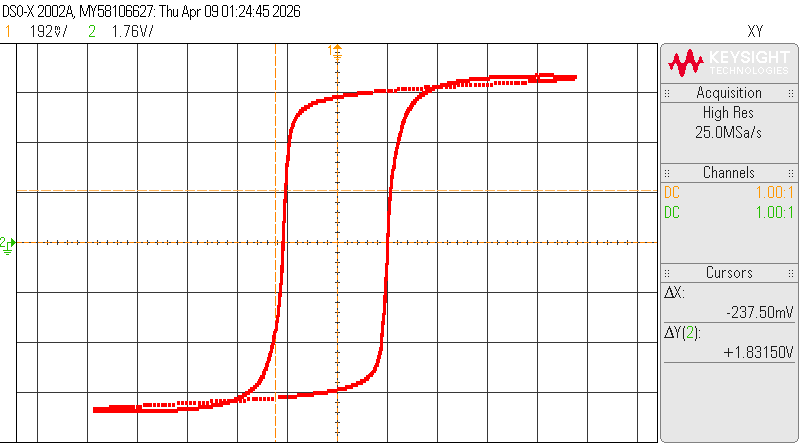
\includegraphics[width=0.90\textwidth]{img/scope_1.png}
\caption{Hysterezní smyčka se zapojeným $R_1$}
\label{fig:r1}
\end{figure}

\begin{figure}[H]
\centering
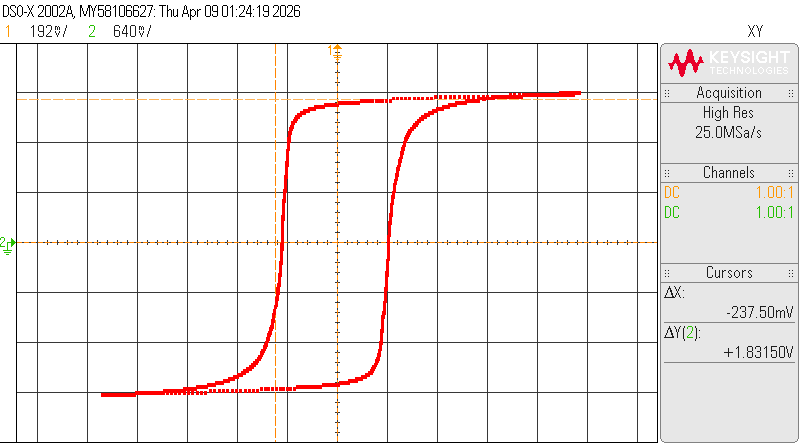
\includegraphics[width=0.90\textwidth]{img/scope_0.png}
\caption{Hysterezní smyčka se zapojeným $R_2$}
\label{fig:r2}
\end{figure}

\begin{figure}[H]
\centering
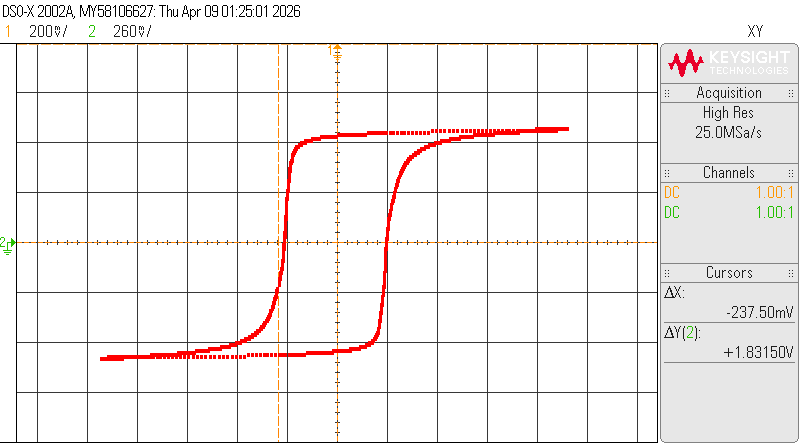
\includegraphics[width=0.90\textwidth]{img/scope_2.png}
\caption{Hysterezní smyčka se zapojeným $R_3$}
\label{fig:r3}
\end{figure}

Jak lze vidět, jako nejvhodnější nám vyšel rezistor $R_2$, protože je smyčka nejčistější. 

\subsubsection{Výpočty}
Z naměřené hodnoty $I_m$ a zadaných parametrů vzorku určete hodnotu $H_m$. Odečtem z osciloskopu zjistěte
hodnotu remanence $B_r$ a koercitivity $H_c$.
\par\noindent\rule{\textwidth}{0.4pt}

$I_m$ jsme určili měřením peak-to-peak napětí na rezistoru $R_4=1\ \Omega$. Naměřili jsme $U_{pp} = 2,56\ V$, z čehož plyne proud:
$$
I_m = \frac{U_{pp}}{2R} = 1,28\ A.
$$

Maximální hodnotu intenzity magnetického pole $H_m$ určíme podle vztahu:
$$
H_m = \frac{N_1 I_m}{l_s}.
$$

Kde střední délku siločáry $l_s$ určíme z vnitřního a vnějšího průměru jádra $(D_1 = 50\ \mathrm{mm},\ D_2 = 98\ \mathrm{mm})$:
$$
l_s = \pi \frac{D_1 + D_2}{2}
= \pi \frac{0,050 + 0,098}{2}
\approx 0,2325\ \mathrm{m}.
$$

Tedy:
$$
H_m = \frac{34 \cdot 1,28}{0,2325} \approx 187\ \mathrm{A\,m^{-1}}.
$$

Remanence $B_r$ je vlastně hodnota magnetické indukce při $H=0$. Určíme ji jako:
$$
B_r = B_m \frac{Y_1}{Y_2}.
$$
Kde $B_m = 1,75\ T$ známe a $Y_1 = 1,80\ V$ je napětí od $(0,0)$ do průsečíku hysterezního obrazce s osou Y (šipka 1) a $Y_2 = 1,93\ V$ je napětí vrcholu smyčky (šipka 2). Po dosazení získáme:
$$
B_r = 1{,}75 \cdot \frac{1{,}80}{1{,}93} \approx 1{,}63\ \mathrm{T}.
$$

Koercitivita $H_c$ je intenzita magnetického pole, která je potřeba, aby se magnetická indukce snížila na nulu. Určíme ji jako:
$$
H_c = H_m \frac{X_1}{X_2}.
$$
Kde $H_m = 187\ \mathrm{A\,m^{-1}}$ jsme vypočítali v předchozím kroku, $X_2 = 1,014\ V$ je x-ová vzdálenost k vrcholu smyčky (šipka 3) a $X_1 = 0,211\ V$ je vzdálenost průsečíku smyčky s osou x (šipka 4). Po dosazení:
$$
H_c = 187 \cdot \frac{0,211}{1,014} \approx 39\ \mathrm{A\,m^{-1}}.
$$

\begin{figure}[H]
\centering
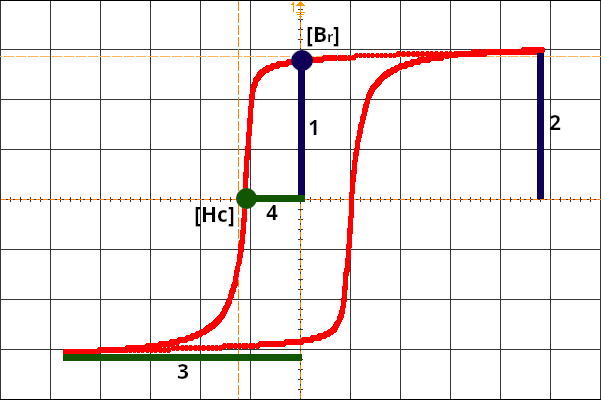
\includegraphics[width=0.90\textwidth]{img/sipky.png}
\caption{Měřené údaje z hysterezní smyčky}
\label{fig:sipky}
\end{figure}

\end{document}
